\documentclass[a4paper, 12pt]{article}
\usepackage[total={17cm,25cm}, top=2.5cm, left=2.5cm, right=2.5cm,  includefoot]{geometry}
\usepackage[utf8]{inputenc}
\usepackage{array}
\usepackage{multirow}
\usepackage{hhline}
\usepackage{gensymb}
\usepackage{graphicx}
\graphicspath{ {} }
\usepackage[czech]{babel}
\usepackage{enumitem}
\usepackage{pdfpages}
\usepackage{amsmath}
\usepackage{verbatim}
\usepackage{listings}
\usepackage{hyperref}
\usepackage{amssymb}


\pagestyle{empty} % vypne číslování stránek




\usepackage[OT2,OT1]{fontenc}
\newcommand\cyr
{
\renewcommand\rmdefault{wncyr}
\renewcommand\sfdefault{wncyss}
\renewcommand\encodingdefault{OT2}
\normalfont
\selectfont
}
\DeclareTextFontCommand{\textcyr}{\cyr}
\def\cprime{\char"7E }
\def\cdprime{\char"7F }
\def\eoborotnoye{\char’013}
\def\Eoborotnoye{\char’003}


\begin{document}



\begin{titlepage}
\begin{center}
\noindent
\Large \textbf{České vysoké učení technické v Praze }\\ Fakulta stavební
\vspace{5cm}

\huge

%vložení loga cvut
\begin{figure}[h!]
	\centering
	
\includegraphics[width=7cm]{logo.png}
\end{figure}

\vspace{0.5cm}

Algoritmy v digitální kartografii \\

\vspace{3cm}

\Huge  
Konvexní obálky\\

\vspace{2cm}

\Large
Bc. Petra Pasovská \\
Bc. David Zahradník \\

\end{center}

\end{titlepage}




\pagestyle{plain}     % zapne obyčejné číslování
\setcounter{page}{1}  % nastaví čítač stránek znovu od jedné

\tableofcontents
\newpage

\section{Zadání}
Níže uvedené zadání je kopie ze stránek předmětu. 

\begin{figure}[h!]
	\centering
	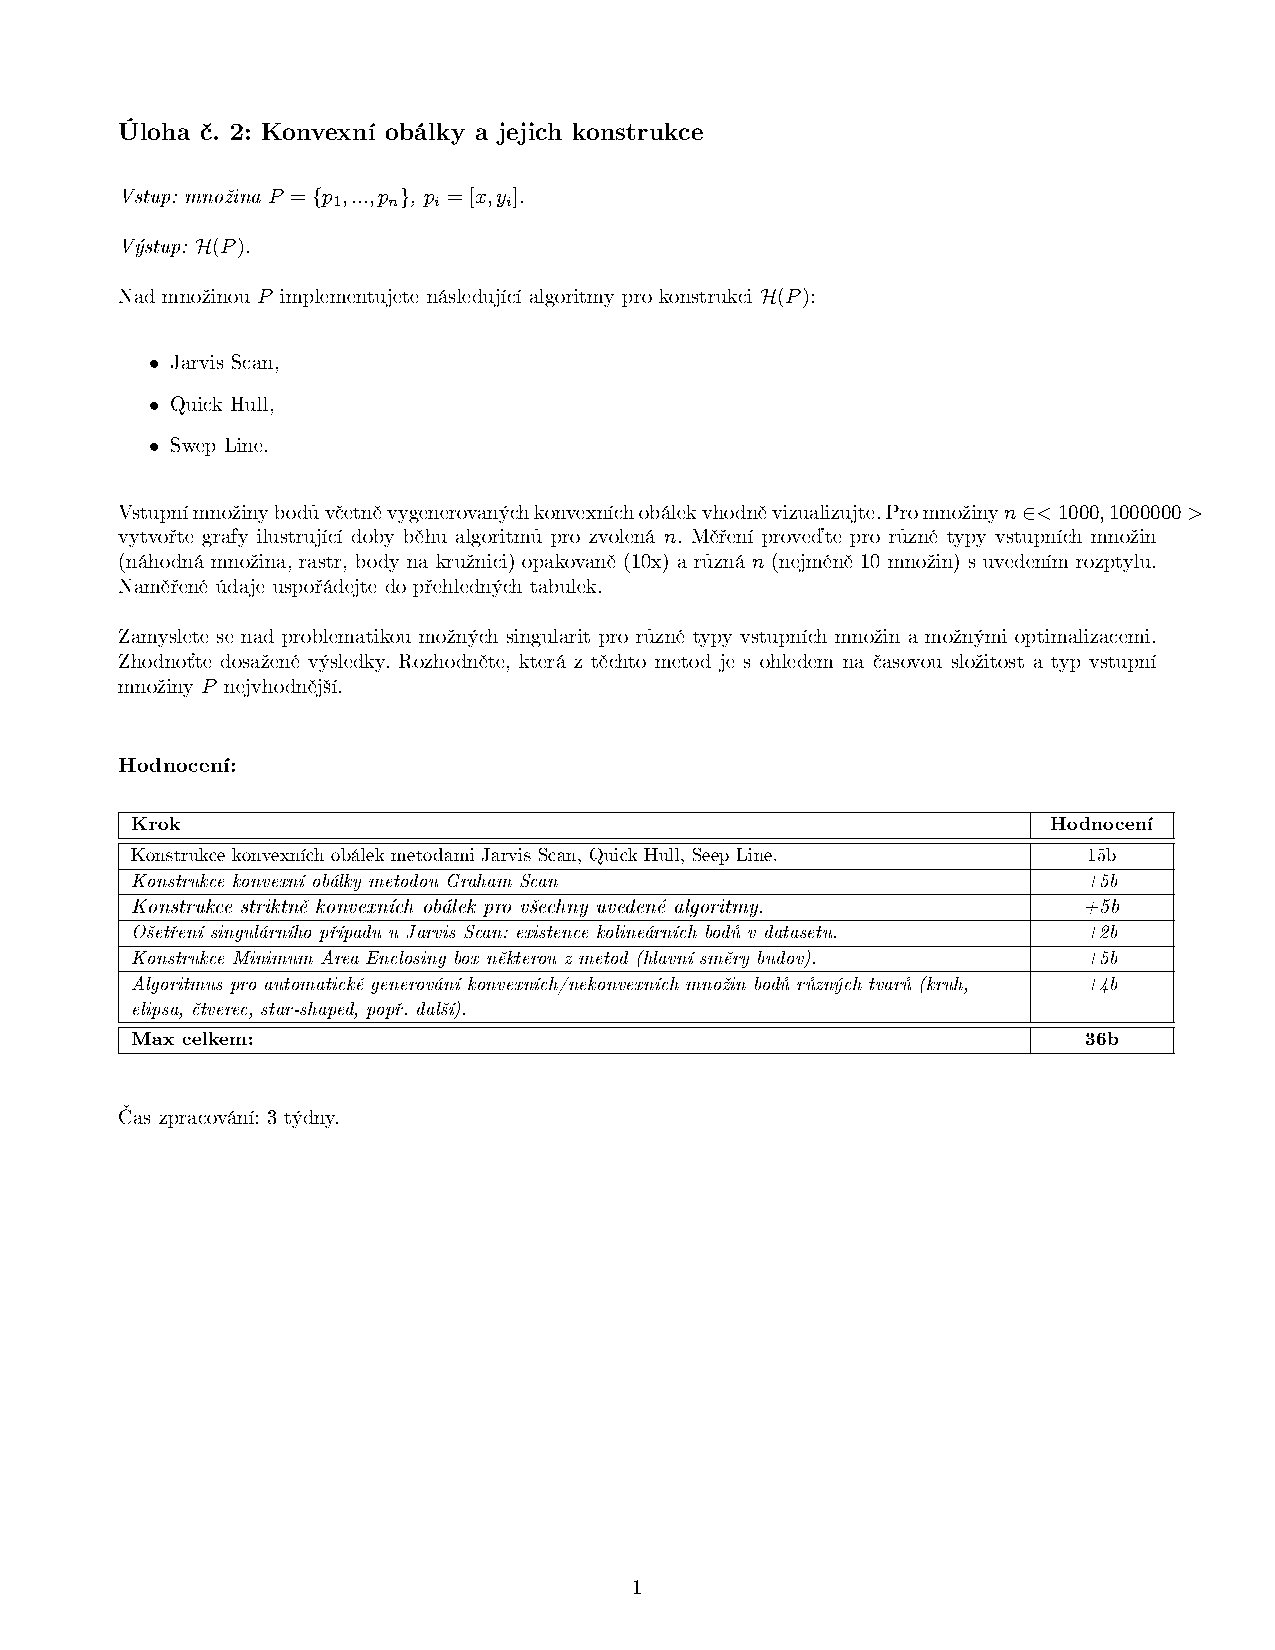
\includegraphics[clip, trim=0cm 10cm 0cm 3cm, width=1.2\textwidth]{zadani.pdf}
\end{figure}

\subsection{Údaje o bonusových úlohách}



\clearpage

\section{Popis a rozbor problému}
Hlavním cílem této úlohy je tvorba aplikace, která pro vygenerované množství bodů vytvoří konvexní obálku za pomoci různých algoritmů. Pro jednotlivé metody byla zapisována i doba trvání algoritmu. Výsledné časy jsou v závěru následně porovnány.\\
\\
Lze říci, že konvexní obálka množiny M je nejmenší konvexní množina, která množinu M obsahuje. V současné době mají konvexní obálky, v některých literaturách označovány jako konvexní obaly, mnoho využití. Často se využívají jako první odhad tvaru nějakého prostorového jevu, např. detekce kolizí, detekce natočení budov a jejich tvaru v kartografii, analýza shluků atd. [Zdroj: 1]
\\

\begin{figure}[h!]
	\centering
	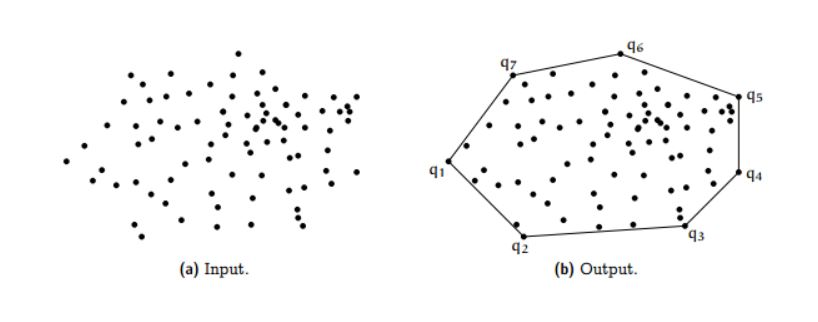
\includegraphics[width=9cm]{convex_hull.jpg}
	\caption{Ukázka vstupních bodů, kolem nichž je vytvořena konvexní obálka. [zdroj: 2]}
\end{figure}

Konvexní obálky využívá celá řada vědních oborů. Zajímavé bylo využití konvexních obálek v paleontologii, kde za pomoci konvexních obálek jsou vědci schopni určit přibližně tvar těla vyhynulých živočichů, jejichž kosti byly nalezeny. \\

\begin{figure}[h!]
	\centering
	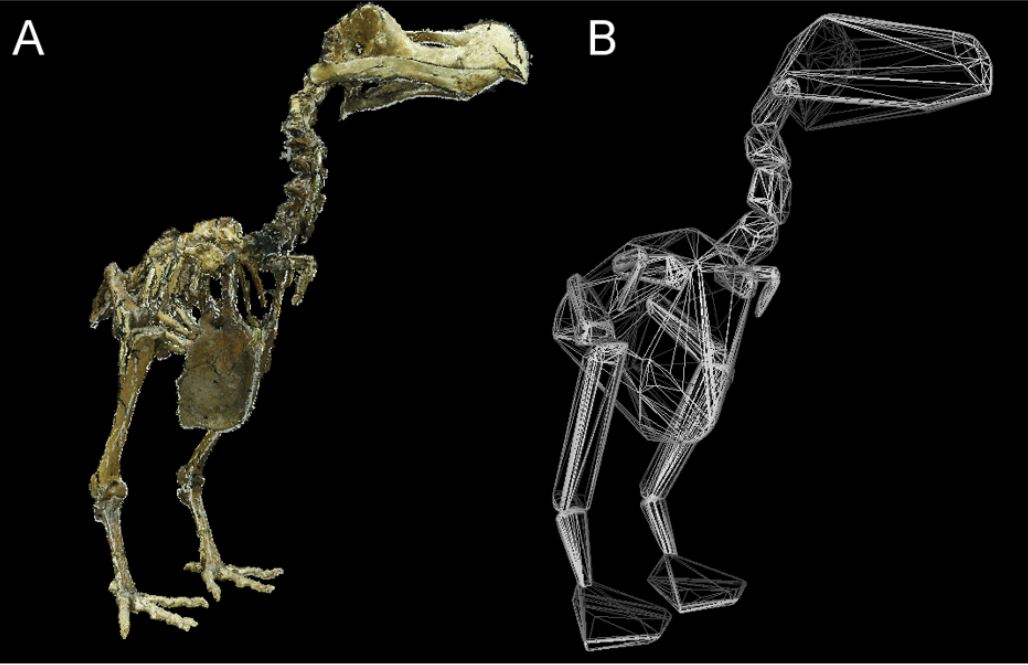
\includegraphics[width=10cm]{paleontology.jpg}
	\caption{Využití konvexních obálek v paleontologii [zdroj: 3]}
\end{figure}


\section{Popis použitých algoritmů}
Existuje několik způsobů jak vytvořit konvexní obálku. V této úloze byly použity pro tovrbu 3 metody. ( 4 když se povede bonus????)

\subsection{Jarvis Scan}
Tato metoda bývá přirovnávána ke způsobu balení dárků (alternativní název Gift Wrapping Algorithm). Předpokladem pro algoritmus Jarvis Scan je, že 3 body nesmí ležet na jedné přímce. Metoda je poměrně snadná pro zápis, velkou nevýhodou je však časová náročnost O($n^2$), které lze dosáhnout, pokud body z množiny S leží na kružnici. Běžný čas výpočtu bývá O(n*h), kde n je počet vstupních bodů a h je počet bodů, které tvoří obálku. [zdroj: 1]\\
\\
Metoda je pojmenována po R. A. Jarvisu, který ji publikoval v roce 1973. \\
\\
Abychom byli schopni algoritmus sestavit, je potřeba nalézt pivot, označme jej q. Nalezení pivota má časovou náročnost O(n). Pivota nalezneme jako bod s minimální hodnotou souřadnice Y. Následně porovnáváme úhel, který svírá pivot a bod následující a předcházející pivotu, dokud nenalezneme maximální úhel. Když takovýto úhel nalezeneme, je přidán mezi body konvexní obálky. V algoritmu dojde k přeindexování bodů a jsou porovnávány následující body, dokud nově vložený bod není pivot. 

\subsubsection{Problematické situace}
K chybě v algoritmu může dojít v případě, že tři body budou kolineární. Tedy v případě, že se budou tři body nacházet na jedné přímce. (Jak bychom toto vyřešili hmm??)


\subsubsection{Implementace metody}
\begin{enumerate}
\item Nalezení pivota q:  $ q = min(y_i) $ 
\item Přidej bod q do konvexní obálky:  $ q \rightarrow H  $ 
\item Inicializuj: $p_j = q; p_{j+1} = p_{j-1}$
\item Opakuj, dokud: $ p_{j+1} \ne q $
\subitem Nalezni $p_{j+1}$: $ p_{j+1} = arg  max_{\forall p_i \in P}  \angle (p_{j-1}, p_j, p_i)$
\subitem Přidej $p_{j+1}$: $ p_{j+1} \rightarrow H  $
\subitem Přeindexování bodů: $ p_{j-1} = p_j; p_j = p_{j+1}  $
\end{enumerate}


\section{Vstupní data}


\section{Výstupní data}


\section{Aplikace}



\section{Dokumentace}



 
\clearpage
\section{Závěr}



\clearpage
\section{Reference}

\begin{enumerate}
\item  MARTÍNEK, Petr. Konvexní obálka rozsáhlé množiny bodů v E\^d [online][cit. 31.10.2018]. \\
Dostupné z: http://graphics.zcu.cz/files/86\_BP\_2010\_Martinek\_Petr.pdf  \\

\item Convex Hulls: Explained. [online][cit. 31.10.2018]\\
Dostupné z: https://medium.com/@harshitsikchi/convex-hulls-explained-baab662c4e94\\

\item Convex-hull mass estimates of the dodo (Raphus cucullatus). [online][cit. 31.10.2018]\\
Dostupné z: https://www.semanticscholar.org/paper/Convex-hull-mass-estimates-of-the-dodo-(Raphus-of-a-Brassey-O\'Mahoney/12e07d3b712561cad16501ac8096120e14901eb8


\end{enumerate}
\end{document}



 